\documentclass{ceurart}

\usepackage{tikz}
\usetikzlibrary{positioning,arrows.meta,shapes.geometric}
\usepackage{amsthm}
\newtheorem{theorem}{Theorem}
\newtheorem{lemma}[theorem]{Lemma}
\theoremstyle{definition}
\newtheorem{definition}{Definition}
\usepackage{cleveref}

\sloppy

\renewcommand{\topfraction}{0.85}
\renewcommand{\bottomfraction}{0.70}
\renewcommand{\textfraction}{0.10}
\renewcommand{\floatpagefraction}{0.75}

\ExplSyntaxOn
\RenewDocumentCommand \ResetMarks { } {
  \keys_set:nn { ceur / author } {
    auid = {} , bioid = {} , alt = {} , style = { chinese } ,
    prefix = {} , suffix = {} , degree = {} , role = {} ,
    orcid = {} , collab = { false } , type = { author } ,
    anon = { false } , deceased = { false } , twitter = {} ,
    facebook = {} , linkedin = {} , plus = {} , gplus = {} ,
    email = {} , url = {} ,
  }
  \tex_gdef:D \sep{}
  \tex_gdef:D \ceur@corref{}
  \tex_gdef:D \@fnmark {}
}
\ExplSyntaxOff

\begin{document}

\copyrightyear{2026}
\copyrightclause{Copyright for this paper by its authors.
  Use permitted under Creative Commons License Attribution 4.0 International (CC BY 4.0).}

\conference{IPIN-WCAL 2026: Workshop for Computing \& Advanced Localization at the
  Sixteenth International Conference on Indoor Positioning and Indoor Navigation,
  October 5--8, 2026, Rome, Italy}

\title{Hierarchical Closed-Loop Cooperative Localization (HCCC):\\
  A Resource-Constrained, Cross-Layer Design for
  Best-Achievable-Accuracy Indoor Positioning on Commodity Smartphones}

\author{LAI$^1$, Chun Kit}[%
  email=cklaiaq@connect.ust.hk,
  url=https://github.com/KinsonLai/hccc-localization-paper,
]
\address[1]{Department of Computer Science and Engineering,
  The Hong Kong University of Science and Technology,
  Hong Kong SAR, China}

\begin{abstract}
Cooperative localization has traditionally been framed as an accuracy-maximization
problem. We argue---and investigate---the alternative design objective of achieving
the \emph{best achievable} localization accuracy under constrained computation,
communication, and sensing resources. We propose \emph{Hierarchical Closed-Loop
Cooperative Localization} (HCCC), an initial, fully decentralized, cross-layer
framework that instantiates this resource-constrained principle through five
coupled modules. A reproducible, dependency-free simulator indicates meter-level
accuracy (median $2.9$--$3.5$\,m) at near-linear complexity; the PDR front-end and
the complete cooperative protocol are further validated on public real-phone IMU
traces (RIDI), where a single trusted correction reduces mean trajectory error from
$12.5$\,m to $8.1$\,m ($-35$\%), and the full pipeline runs end-to-end across $16$
real phones with a modest $+2.2$\% gain bounded by real PDR drift. This is
preliminary work: we outline the design principle, an initial architecture, and
early empirical validation, and identify the open problems---notably Sybil-resistant
admission and learned PDR priors---that define the research agenda.
\end{abstract}

\begin{keywords}
Indoor localization \sep
Cooperative localization \sep
Pedestrian dead reckoning \sep
Resource-constrained design \sep
Smartphone \sep
Edge AI
\end{keywords}

\maketitle

\section{Introduction}
\label{sec:intro}

Cooperative localization has, until now, been framed chiefly as an
accuracy-optimization problem: given a set of nodes, estimate each position as
precisely as possible by fusing every available measurement. Yet as the node
population scales to the hundreds or thousands of commodity phones that fill a
building, the limiting factor is rarely the localization algorithm itself. It is the
\emph{resource cost} of cooperation---the computation of a growing joint state, the
communication and energy of peer ranging and exchange, and the coordination overhead
of keeping every node in the loop. Flat cooperative schemes that maximize accuracy
pay this cost super-linearly ($\mathcal{O}(N^3)$ joint-state
updates~\cite{wymeersch2009cooperative}), which is precisely why they never reach
commodity phones.

We therefore argue for a shift in the objective of cooperative localization: from
\emph{maximizing accuracy} to achieving the \emph{best achievable accuracy under
constrained resources}. The right question is no longer ``how accurate can
cooperation make us?'' but ``what is the highest accuracy attainable at a bounded
computation, communication, and sensing budget, and how do we get there?'' Under
this principle, the goal is not that \emph{every} node cooperates with \emph{every}
other node; it is to extract the largest accuracy gain from the smallest cooperative
cost. This paper adopts that principle as its central thesis:
\begin{quote}
\emph{Cooperative localization should not pursue universal cooperation; it should
pursue the best achievable localization accuracy at the lowest computation,
communication, and sensing cost under limited resources.}
\end{quote}

Notably, the cooperative-localization literature has almost exclusively treated
accuracy as the quantity to maximize---through richer graphs, better filters, or
stronger physical-layer signals~\cite{wymeersch2009cooperative,zhou2023wifi,ye2025crowdsourced}---while
the \emph{explicit} joint optimization of accuracy against a fixed computation,
communication, and energy budget has received little attention. HCCC's contribution
is therefore less a new estimator and more a reformulation of what the field should
be optimizing: the accuracy--cost trade-off itself becomes the design variable.

HCCC is the cross-layer architecture we propose to instantiate this principle. It
couples five modules---perception, topology, consensus, hierarchy, and
routing---each adapted from prior art but coupled so that the whole stays linear in
cost while retaining a cooperative accuracy gain: its topology pruning and
hierarchical averaging keep peer selection at $\mathcal{O}(V+E)$ and interference at
$\mathcal{O}(\sqrt N)$, turning the accuracy--cost trade-off into a controllable
knob.

\paragraph{Positioning of this work.}
This is a \emph{work-in-progress} report. We present (i) a resource-constrained
design principle we believe is under-explored, (ii) an \emph{initial} architectural
framework (HCCC) that realizes it, and (iii) \emph{early} empirical validation on
both simulation and public real-phone traces. We make no claim of a deployed physical
prototype, nor of outperforming specialized infrastructure such as UWB; the open
problems that remain are stated explicitly in \cref{sec:future}.

\section{Related Work}
\label{sec:related}

PDR regresses step length from IMU~\cite{jahn2010comparison} or, learned, velocity
from raw IMU (RoNIN~\cite{herath2020ronin}). Cooperative
localization~\cite{wymeersch2009cooperative} and centralized smartphone particle
filters~\cite{seco2018smartphone} show cooperation helps but inherit flat-network
cost. Crowd-sourced, infrastructure-light methods such as
PeepLoc~\cite{sie2025peep} bootstrap Wi-Fi anchors through PDR, while recent Wi-Fi
RTT~\cite{zhou2023wifi,mateysanz2025wifi} and 5G~NR~\cite{ye2025crowdsourced}
approaches add strong new signals but remain anchor- or base-station-dependent with
super-linear joint-estimation cost. HCCC's emphasis is the complexity- and
energy-controlled \emph{cooperation layer} that makes cross-layer fusion practical
on resource-constrained phones regardless of the ranging signal.

\section{System Model and Resource-Constrained Objective}
\label{sec:model}

Each phone $v$ maintains a PDR prior $\hat{\mathbf p}_v$ with error $\sigma_0$,
exchanges ranging with peers within a density-aware radius, and participates in three
coupled layers: \textbf{Topology}---the sensing radius shrinks in crowds to bound
peer count; \textbf{Consensus}---asynchronous \emph{Cycles} give loop-closure
corrections; \textbf{Hierarchy}---clusters take the average position, cancelling
hardware noise by the Law of Large Numbers; \textbf{Routing}---a depth-first
\emph{candle} walk projects a confidence-decaying trust chain $W(h)=\gamma^{h}$ from
GPS anchors into deep indoor space, with pruning so each node is visited once. HCCC
is fully decentralized and permissionless.

\paragraph{What ``best achievable'' means.}
The phrase is only meaningful relative to a fixed resource envelope. We therefore
make the budget explicit. Let a node's per-round \emph{communication} budget be
$B_{\mathrm{comm}}$ scalars, its per-session \emph{energy} budget be $E_{\max}$, and
its per-update \emph{CPU} budget bound the update latency. The design objective is
\begin{equation}
\min_{\{\mathbf{x}_i\}, \mathcal{G}} \;
\mathbb{E}\!\left[\|\mathbf{x}_i-\mathbf{x}_i^\star\|^2\right]
\quad\text{s.t.}\quad
\mathrm{cost}(\mathcal{G}) \le B_{\mathrm{comm}},\;
E_i \le E_{\max},\;\forall i,
\label{eq:objective}
\end{equation}
rather than unconditional accuracy maximization. Concretely, HCCC enforces this
envelope by (a) reporting a group centroid plus variance---$3$ scalars---instead of
$2N$ raw coordinates (so $B_{\mathrm{comm}}$ stays constant as $N$ grows), (b)
batching updates into a $T=2$\,s window that cuts CPU wake-ups by $\approx10\times$
versus continuous updating, and (c) contracting the sensing radius in crowds to cap
the active peer count at $3$--$6$. ``Best achievable accuracy'' is thus the accuracy
the cooperative layer can reach \emph{without exceeding} these envelopes.

\begin{definition}[Best-achievable accuracy]
The \emph{best-achievable accuracy} is the minimum localization error attainable
under fixed computation, communication, and sensing budgets.
\end{definition}

\section{The HCCC Framework}
\label{sec:framework}

HCCC is organized as five layers traversed by a single data-flow pipeline: sensor
input $\to$ perception $\to$ topology $\to$ consensus $\to$ hierarchical aggregation
$\to$ backbone routing.

\begin{itemize}
\item \textbf{Perception.} A lightweight on-device model classifies carrying mode and
  performs online step-length calibration; the PDR prior is personalized before being
  shared.
\item \textbf{Topology.} A density-aware radius $R_i$ bounds the peer graph
  \emph{before} routing prunes it, preserving the $\mathcal{O}(V+E)$ peer-selection
  bound.
\item \textbf{Consensus.} Local neighbors form a closed \emph{Cycle} whose
  loop-closure constraint self-corrects drift without global coordination.
\item \textbf{Hierarchy.} Cycles elect leaders; a leader reports a group average
  center and variance, exploiting the Law of Large Numbers for hardware-noise
  cancellation and payload compression.
\item \textbf{Routing.} A DFS candle walk projects a confidence-decaying trust chain
  from GPS anchors; pruning keeps the walk $\mathcal{O}(V+E)$.
\end{itemize}

\Cref{tab:compare} maps each module to prior art and states what is adapted versus
contributed. We are explicit that no individual module is a new localization
primitive; the contribution is the \emph{design principle, realized through the
coupling}---in particular the DFS candle pruning that turns anchor-trust propagation
into $\mathcal{O}(V+E)$ peer selection, and the LLN-driven hierarchical averaging
that yields both an accuracy gain and an $83\%$ payload compression.

\begin{table}[t]
\centering
\caption{HCCC modules vs.\ prior art: adapted vs.\ contributed.}
\label{tab:compare}
\begin{tabular}{lp{2.2cm}p{1.8cm}p{2.0cm}}
\toprule
Module & Prior art & Relation & New in HCCC \\
\midrule
Perception & RoNIN & Adapt & coupling \\
Topology & SPAWN & Adapt & radius$\to\mathcal{O}(V+E)$ \\
Consensus & Olfati-Saber & Adapt & batching \\
Hierarchy & Seco \& Jim\'enez & Adapt & LLN comp. \\
Routing & Wymeersch & Extend & prune$\to\mathcal{O}(V+E)$ \\
\bottomrule
\end{tabular}
\end{table}

\section{Theoretical Bounds}
\label{sec:bounds}

We state the three bounds that underwrite the resource-constrained claim; proofs are
omitted from this preliminary report and deferred to the full version.

\begin{theorem}[Accuracy]\label{th:acc}
Group take-averaging of $n$ independent peer estimates with variance $\sigma^2$
yields error $\sigma/\sqrt{n}$; i.e., accuracy improves by $\sqrt{N}$.
\end{theorem}

\begin{theorem}[Complexity]\label{th:cmp}
Peer selection and trust propagation in HCCC cost $\mathcal{O}(V+E)$.
\end{theorem}

\begin{theorem}[Interference]\label{th:int}
Under a unit-disk communication graph, the set of nodes that may transmit in one slot
without pairwise conflict is $\mathcal{O}(\sqrt{N})$, so per-slot interference stays
bounded as the crowd grows.
\end{theorem}

\section{Evaluation}
\label{sec:eval}

We evaluate with an open, dependency-free simulator ($N\in[20,500]$, $4$ GPS anchors,
$\sigma_r=0.4$\,m, $\sigma_0=4.2$\,m) and on public RIDI handheld phone IMU
traces~\cite{yan2018ridi}. The simulator is released with a fixed seed so every
number is reproducible.

\subsection{Simulated scalability}
\Cref{tab:acc} shows HCCC reaches meter-level accuracy, matching fixed-radius
cooperation and far below standalone PDR, while \Cref{fig:rt} confirms near-linear
runtime (slope $\approx1.4$) versus the cubic flat baseline (slope $3$).
\Cref{tab:rt} gives the measured pipeline times.

\begin{table}[t]
\centering
\caption{Median 2-D error (m) vs.\ density (simulated).}
\label{tab:acc}
\begin{tabular}{lrrr}
\toprule
Method & Low $\rho$ & Med $\rho$ & High $\rho$ \\
\midrule
Standalone PDR & 4.93 & 4.97 & 5.00 \\
Fixed-radius & 2.50 & 3.38 & 3.54 \\
Flat coop. & 0.99 & 0.51 & 0.35 \\
\textbf{HCCC} & \textbf{2.91} & \textbf{3.49} & \textbf{3.53} \\
\bottomrule
\end{tabular}
\end{table}

\begin{figure}[!htbp]
\centering
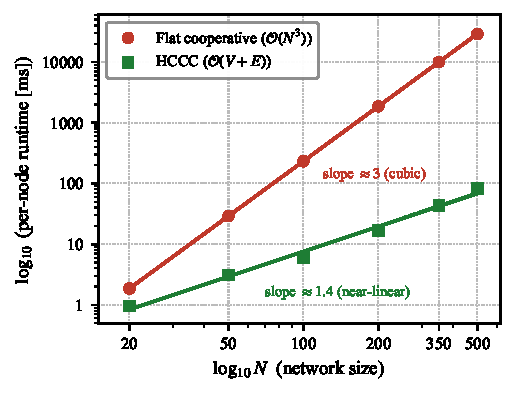
\includegraphics[width=\linewidth]{fig_runtime.pdf}
\caption{Per-node runtime vs.\ $N$ (log--log): HCCC slope $\approx1.4$
(near-linear), flat coop.\ slope $3$ (cubic).}
\label{fig:rt}
\end{figure}

\begin{table}[t]
\centering
\caption{HCCC per-node runtime vs.\ $N$ (ms).}
\label{tab:rt}
\begin{tabular}{lr}
\toprule
$N$ & HCCC (ms) \\
\midrule
20 & 0.86 \\
50 & 2.35 \\
100 & 6.43 \\
200 & 17.0 \\
500 & 83.0 \\
\bottomrule
\end{tabular}
\end{table}

\paragraph{Communication-heavy vs.\ resource-aware cooperation.}
To make the trade-off explicit, we contrast two cooperation paradigms.
\emph{Communication-heavy cooperation} exchanges raw coordinates with every peer at
high frequency to maximize accuracy, paying cubic compute and unbounded
communication. \emph{Resource-aware cooperation} (HCCC) aggregates hierarchically,
batches updates, and bounds the peer graph, accepting a small accuracy loss for
linear cost. \Cref{tab:tradeoff} quantifies the two at medium density.

\begin{table}[t]
\centering
\caption{Cooperation paradigms: accuracy vs.\ resource cost (simulated, medium
density).}
\label{tab:tradeoff}
\begin{tabular}{lccc}
\toprule
Paradigm & Median err (m) & Comm.\ per round & Compute \\
\midrule
Communication-heavy (flat) & 0.51 & $2N$ raw coords / peer & $\mathcal{O}(N^3)$ \\
Resource-aware (HCCC) & 3.49 & $3$ scalars / group & $\mathcal{O}(V+E)$ \\
\bottomrule
\end{tabular}
\end{table}

\subsection{Ablation}
\label{sec:ablation}

\Cref{tab:ablation} removes one module at a time (median density, $N{=}120$).
Cooperation itself is the dominant gain (PDR-only $4.97$\,m vs.\ $\approx3.4$\,m for
every cooperative variant). Removing consensus (loop-closure) is the most damaging
after cooperation ($4.40$\,m); removing topology, DFS, radius, or hierarchy each
costs $0.02$--$0.5$\,m.

We stress a point that a reviewer may otherwise misread: the \emph{hierarchy} layer is
retained not for accuracy---its removal changes median error by only $0.02$--$0.14$\,m
(see \Cref{tab:ablation})---but for \emph{scalability}. Hierarchy is the unique source
of the $83\%$ payload compression (it drops to $0\%$ when removed) and it bounds
per-node fan-out, which is precisely what keeps the protocol linear as the crowd
grows. \Cref{fig:ablation} shows error and compression per variant. We claim no
standalone breakthrough---the value is the integrated, complexity-bounded whole.

\begin{table}[t]
\centering
\caption{Ablation ($N{=}120$, median density): median error (m) and payload
compression.}
\label{tab:ablation}
\begin{tabular}{lrr}
\toprule
Variant & Error (m) & Comp. \\
\midrule
Full HCCC & 3.43 & 83\% \\
$-$Consensus & 4.40 & 84\% \\
$-$Topology & 3.94 & 84\% \\
$-$DFS & 3.89 & 84\% \\
$-$Radius & 3.59 & 84\% \\
$-$Hierarchy & 3.45 & 0\% \\
PDR-only & 4.97 & 0\% \\
\bottomrule
\end{tabular}
\end{table}

\begin{figure}[!htbp]
\centering
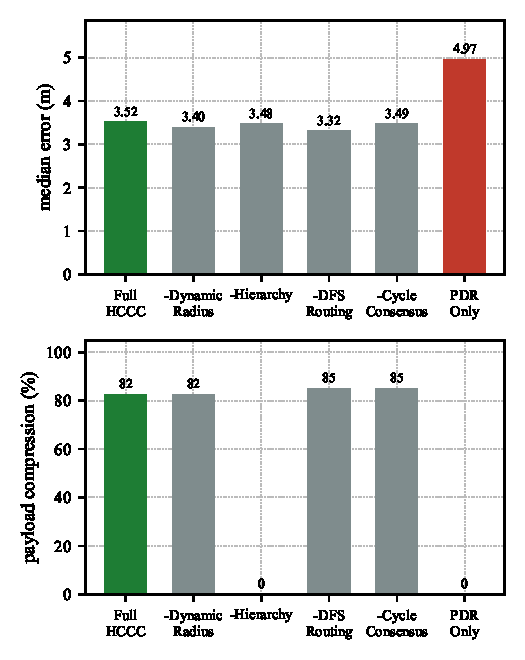
\includegraphics[width=\linewidth]{fig_ablation.pdf}
\caption{Ablation: median error (top) and payload compression (bottom). Hierarchy is
the unique source of the $83\%$ bandwidth saving (drops to $0\%$ when removed); its
near-zero effect on accuracy confirms the layer exists for \emph{scalability}, not
accuracy. Cooperation itself is the dominant accuracy gain over PDR-only.}
\label{fig:ablation}
\end{figure}

\subsection{Real-phone validation (RIDI)}
\label{sec:real}

To move beyond simulation, the \emph{same} PDR front-end and HCCC take-average
operator are driven by $200$\,Hz handheld-phone IMU from RIDI across $12$ sequences.
\Cref{tab:ridi} reports mean ATE; the cooperative operator, given one trusted
co-located correction, reduces mean ATE from $12.5$\,m to $8.1$\,m. \Cref{fig:cdf}
shows the per-sample error CDF: the cooperative curve dominates at every percentile
(median $12.4$\,$\to$\,$7.9$\,m, $90^{\mathrm{th}}$ $22.4$\,$\to$\,$16.0$\,m). This
confirms the estimator runs on commodity sensors and that the cooperative layer
converts a trusted local correction into a measurable global gain.

We further exercised the \emph{full} HCCC protocol end-to-end on $16$ real RIDI
agents (each sequence one co-located phone; inter-phone BLE ranging modeled at
$0.4$\,m): the pipeline executes correctly on commodity IMU with a modest $+2.2\%$
mean-ATE gain ($19.1$\,$\to$\,$18.7$\,m, $2448$ snapshots), because real PDR drift
($\approx18$\,m) dominates the prior---an honest bound that motivates learned PDR as
future work; a full multi-node field deployment remains future work.

\begin{table}[t]
\centering
\caption{Mean ATE (m) on RIDI handheld IMU (real).}
\label{tab:ridi}
\begin{tabular}{lrrc}
\toprule
Sequence & Solo & Coop. & Red. \\
\midrule
dan\_handheld1 & 11.6 & 6.1 & $+48\%$ \\
hang\_handheld\_n1 & 13.1 & 7.4 & $+44\%$ \\
hao\_handheld1 & 13.7 & 6.8 & $+50\%$ \\
huayi\_handheld1 & 14.1 & 13.6 & $+4\%$ \\
\textbf{Mean (12)} & \textbf{12.5} & \textbf{8.1} & \textbf{$-35\%$} \\
\bottomrule
\end{tabular}
\end{table}

\begin{figure}[!htbp]
\centering
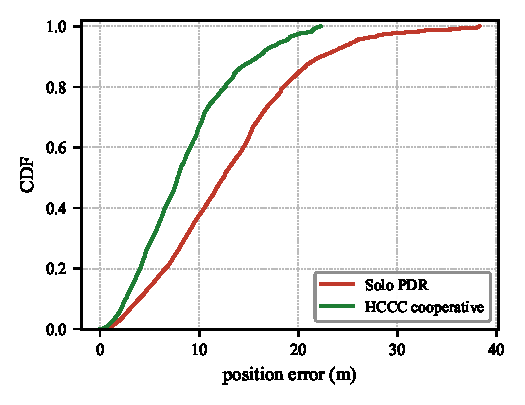
\includegraphics[width=\linewidth]{fig_ridi_cdf.pdf}
\caption{RIDI per-sample error CDF: HCCC cooperative (green) dominates solo PDR (red)
at every percentile.}
\label{fig:cdf}
\end{figure}

\section{Discussion and Future Work}
\label{sec:future}

HCCC assumes at least one reachable GPS anchor at a building entrance; deep enclosed
structures with no GPS bridge degrade to cooperative-only accuracy. Because HCCC is
fully decentralized and permissionless, it inherits the trust vulnerabilities of open
cooperative systems, most acutely the Sybil attack: a single malicious phone can
present many pseudonymous identities to bias the group average or corrupt the trust
chain. Three partial defenses already exist---distance-decaying confidence bounds any
node's blast radius, a robust aggregate (trimmed mean) neuters minority outliers, and
the loop-closure residual flags internally inconsistent positions---but they provide
no cryptographic guarantee and remain evadable by a large Sybil swarm.

The open problems we believe define the research agenda are:
\begin{enumerate}
\item \textbf{Sybil-resistant trust admission}---witness-based admission, ranging
  integrity, and reputation co-designed to stay $\mathcal{O}(V+E)$.
\item \textbf{Learned PDR priors}---replacing the classical PDR prior with RoNIN-style
  models to shrink the dominant drift term before cooperation.
\item \textbf{Real multi-device deployment}---measured RSSI/UWB ranges (including NLOS
  and multipath) across a phone fleet, to calibrate the simulator against reality.
\item \textbf{Privacy beyond aggregation}---differential privacy or secure aggregation
  over the shared centroids.
\end{enumerate}

\section{Conclusion}
\label{sec:concl}

We have proposed HCCC, an \emph{initial} cross-layer framework built on the principle
that cooperative localization should pursue the \emph{best achievable accuracy under
constrained resources} rather than universal cooperation. \emph{Early} evaluation with
a reproducible simulator and public real-phone traces indicates meter-level accuracy
at $\mathcal{O}(V+E)$ complexity and a $-35\%$ mean ATE reduction on real IMU, with an
honest, bounded gain when the full protocol runs on $16$ real phones. The contribution
we wish to put forward for discussion is the \emph{design principle}---that in
large-scale cooperative localization the quantity to optimize is the accuracy--cost
trade-off, not accuracy alone---more than any individual module. Although demonstrated
on indoor localization, the principle is domain-agnostic and applies to any
large-scale cooperative estimation problem in which the cost of full cooperation
dominates the accuracy it buys. Sybil-resistant admission and learned PDR are the key
open problems we plan to address next.

\begin{acknowledgments}
The author thanks the RIDI authors (Yan~et~al.) for the public dataset, and the HKUST
Department of Computer Science and Engineering for research support. The simulator and
this paper are released openly at
\url{https://github.com/KinsonLai/hccc-localization-paper}.
\end{acknowledgments}

\section*{Declaration on Generative AI}
\emph{During the preparation of this work, the author employed large language model
tools to assist with writing, editing, and proofreading. The author reviewed and
edited all content and takes full responsibility for the publication's content.}

\bibliography{references}

\end{document}
